\documentclass[../main.tex]{subfiles}
\begin{document}
\chapter{Pengenalan Pengembangan Game dan Unity}

\section{Konsep Dasar Game}
Game adalah sistem interaktif dengan aturan, tujuan, dan umpan balik yang membentuk pengalaman bermain. Dalam pengembangan perangkat lunak, game merepresentasikan dunia simulatif yang berubah sebagai respons terhadap input dan logika yang dirancang, sehingga interoperasi antara mekanika, antarmuka, dan aset menjadi krusial. Perancangan loop inti (core loop)—misalnya siklus mengeksplorasi, beraksi, dan menerima umpan balik—menjadi fondasi keterlibatan pemain yang berkelanjutan \parencite{gpp-nystrom,fullerton2008game}.

Mesin permainan (game engine) menyediakan abstraksi grafis, audio, input, fisika, dan manajemen aset agar tim berfokus pada konten dan mekanika alih-alih subsistem rendah-level. Pemilihan engine memengaruhi alur kerja, kinerja, dan portabilitas produk. Unity banyak dipakai di industri dan pendidikan karena ekosistemnya luas, dokumentasi komprehensif, dan dukungan lintas platform yang matang \parencite{unity-manual-overview,unity-scripting-start-update}.

\section{Genre Game}
Genre menyediakan kerangka untuk mengelompokkan mekanika, ritme permainan, dan ekspektasi pengguna sehingga tim dapat memprioritaskan fitur inti sejak awal. Klasifikasi genre membantu menentukan kebutuhan kamera, antarmuka, dan kontrol interaksi, misalnya perbedaan signifikan antara platformer 2D dan RPG berbasis aksi. Dengan basis ini, perencanaan teknis dan desain dapat disinkronkan sejak tahap praproduksi \parencite{schell2019book}.

Walau genre deskriptif, inovasi mekanika tetap dimungkinkan dengan menggabungkan elemen dari berbagai genre secara terkontrol. Strategi yang efektif ialah memetakan fitur genre ke pola implementasi yang dapat digunakan kembali, seperti objek kolektibel, sistem inventori, atau percabangan misi. Pendekatan berbasis pola memudahkan dokumentasi dan mengurangi risiko teknis saat iterasi \parencite{gpp-nystrom,schell2019book}.

\begin{table}[h]
  \centering
  \caption{Contoh pemetaan genre ke fokus teknis}
  \begin{tabularx}{\textwidth}{@{}lXX@{}}
    \toprule
    Genre & Fokus Mekanika & Implikasi Teknis \\
    \midrule
    Platformer 2D & Lompatan presisi, rintangan & Fisika 2D, deteksi tumbukan, kamera sisi \\
    RPG Aksi & Pertarungan, progres karakter & Sistem status, AI dasar, antarmuka inventori \\
    Puzzle & Tantangan logika & State-space kecil, UI instruktif, telemetri kesulitan \\
    \bottomrule
  \end{tabularx}
\end{table}

\section{Antarmuka dan Proyek Unity}
Editor Unity terdiri atas panel utama seperti \textit{Hierarchy}, \textit{Scene}, \textit{Inspector}, \textit{Project}, dan \textit{Console} yang masing-masing melayani tugas berbeda. \textit{Hierarchy} mengelola struktur objek, \textit{Scene} memberi konteks visual, \textit{Inspector} menyunting properti, \textit{Project} mengatur aset, dan \textit{Console} menampilkan pesan sistem. Pemahaman fungsi tiap panel mempercepat alur kerja dan mengurangi kesalahan konfigurasi saat membangun fitur permainan \parencite{unity-manual-overview}.

Struktur proyek Unity lazim meliputi \textit{Assets}, \textit{Packages}, dan \textit{ProjectSettings} dengan penataan aset yang konsisten untuk kolaborasi. Praktik umum adalah memisahkan \textit{Art}, \textit{Audio}, \textit{Prefabs}, dan \textit{Scenes}, serta mendokumentasikan konvensi impor dan penamaan. Mengikuti struktur yang direkomendasikan dokumentasi resmi membantu menjaga kinerja editor dan kompatibilitas lintas versi \parencite{unity-project-structure}.

\begin{figure}[h]
  \centering
  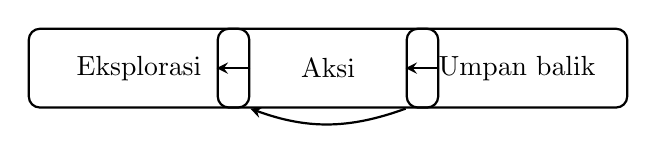
\begin{tikzpicture}[node distance=2.4cm,>=stealth,thick]
    \tikzstyle{state}=[rectangle, draw, rounded corners, minimum width=2.8cm, minimum height=1cm, align=center]
    \node[state] (explore) {Eksplorasi};
    \node[state, right of=explore] (act) {Aksi};
    \node[state, right of=act] (feedback) {Umpan balik};
    \draw[->] (explore) -- (act);
    \draw[->] (act) -- (feedback);
    \draw[->] (feedback) to[bend left=20] node[above] {} (explore);
  \end{tikzpicture}
  \caption{Core loop sederhana: eksplorasi, aksi, dan umpan balik \parencite{gpp-nystrom}.}
\end{figure}

\onlyinsubfile{\printbibliography}
\end{document}
